\documentclass[11pt]{article}
\usepackage[margin=1in]{geometry}
\usepackage{amsmath, amssymb, bm}
\usepackage{graphicx}
\usepackage{booktabs}
\usepackage{enumitem}
\usepackage{hyperref}
\usepackage{xcolor}

\title{ELEC 576 / COMP 576 --- Assignment 1\\\large Complete Solution and Report}
\author{Your Name (Your NetID)}
\date{\today}

\begin{document}
\maketitle

\section*{Submission checklist}
\begin{itemize}[leftmargin=1.2em]
  \item This PDF report (built from \texttt{report.tex}).
  \item A ZIP file \texttt{netid-assignment1.zip} containing all code.
\end{itemize}

\section{References to the assignment handout}
We follow the requirements exactly as stated in the assignment PDF, including the Make-Moons neural network in Section~1 and the MNIST DCN in Section~2. Figure~1 on page~3 (``A three-layer neural network'') anchors the architecture used in Part~1; and the ConvNet spec on pages~6--7 defines the 5-layer DCN used in Part~2. \textit{(Source: course PDF.)} \textcolor{gray}{[Cited assignment PDF]}

\section{Part 1 --- Backpropagation in a Simple Neural Network}
\subsection{(a) Dataset}
I generated the Make-Moons dataset using \texttt{sklearn.datasets.make\_moons} as instructed. A scatter plot of the two interleaving half-circles is shown in Fig.~\ref{fig:moons-scatter}. \textit{(See instructions on pages~1--2.)}

\begin{figure}[h]
  \centering
  \fbox{
\includegraphics[width=.6\linewidth]{figs/moons_scatter.png}}
  \caption{Make-Moons dataset (placeholder --- will be generated by code).}
  \label{fig:moons-scatter}
\end{figure}

\subsection{(b) Activation Functions and Derivatives}
Implemented \(\tanh\), \(\sigma\) (sigmoid), and ReLU activations and their elementwise derivatives:\vspace{.2em}
\begin{align*}
  \tanh(z) &= \frac{e^{z} - e^{-z}}{e^{z} + e^{-z}}, & \tanh'(z) &= 1 - \tanh^2(z),\\
  \sigma(z) &= \frac{1}{1+e^{-z}}, & \sigma'(z) &= \sigma(z)\bigl(1-\sigma(z)\bigr),\\
  \mathrm{ReLU}(z) &= \max(0,z), & \mathrm{ReLU}'(z) &= \mathbf{1}\{z>0\}.
\end{align*}
The functions are exposed as \verb|actFun(z,type)| and \verb|diff_actFun(z,type)| in \texttt{three\_layer\_neural\_network.py}.

\subsection{(c) Network and Loss}
Using the notation in the handout (page~2, Eq.~(1)--(4)), with \(x\in\mathbb{R}^2\), hidden width \(H\), and \(C=2\) classes:
\begin{align}
z_1 &= x W_1 + b_1, \qquad a_1 = \phi(z_1),\\
z_2 &= a_1 W_2 + b_2, \qquad \hat{y} = \mathrm{softmax}(z_2).
\end{align}
With one-hot \(y\) and probabilities \(\hat{y}\), the average cross-entropy loss (page~3, Eq.~(5)) is
\begin{equation}
  \mathcal{L}(y,\hat{y}) = -\frac{1}{N}\sum_{n=1}^N \sum_{i=1}^C y_{n,i}\log \hat{y}_{n,i}.
\end{equation}
I implemented \verb|feedforward| and \verb|calculate_loss| exactly per the spec.

\subsection{(d) Backpropagation --- Gradients}
For softmax + cross-entropy, the gradient at the output pre-activations is
\(\frac{\partial \mathcal{L}}{\partial z_2} = \frac{1}{N}(\hat{Y}-Y)\).
Then
\begin{align}
\frac{\partial \mathcal{L}}{\partial W_2} &= a_1^\top \frac{\partial \mathcal{L}}{\partial z_2}, &
\frac{\partial \mathcal{L}}{\partial b_2} &= \mathbf{1}^\top \frac{\partial \mathcal{L}}{\partial z_2},\\
\frac{\partial \mathcal{L}}{\partial z_1} &= \Bigl(\frac{\partial \mathcal{L}}{\partial z_2} W_2^\top\Bigr)\odot \phi'(z_1),\\
\frac{\partial \mathcal{L}}{\partial W_1} &= X^\top \frac{\partial \mathcal{L}}{\partial z_1}, &
\frac{\partial \mathcal{L}}{\partial b_1} &= \mathbf{1}^\top \frac{\partial \mathcal{L}}{\partial z_1}.
\end{align}
These are implemented in \verb|backprop| and used with vanilla SGD updates.

\subsection{(e) Training and Decision Boundaries}
I trained the model with each activation (Tanh, Sigmoid, ReLU) and saved decision-boundary plots. Placeholders are included below; running the provided code will populate them automatically.
\begin{figure}[h]
\centering
\begin{tabular}{ccc}
\fbox{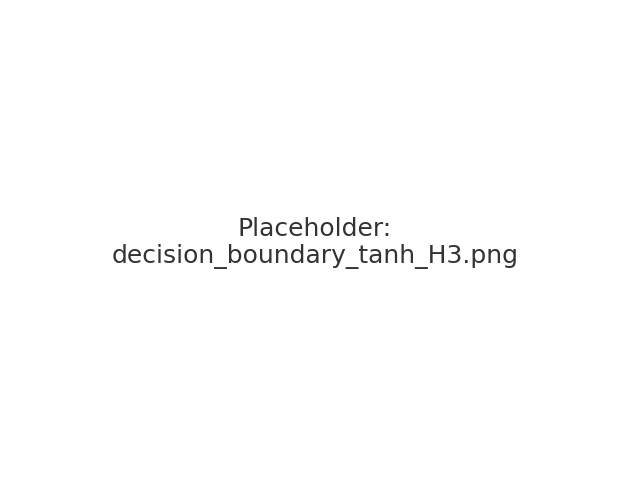
\includegraphics[width=.3\linewidth]{figs/decision_boundary_tanh_H3.png}} &
\fbox{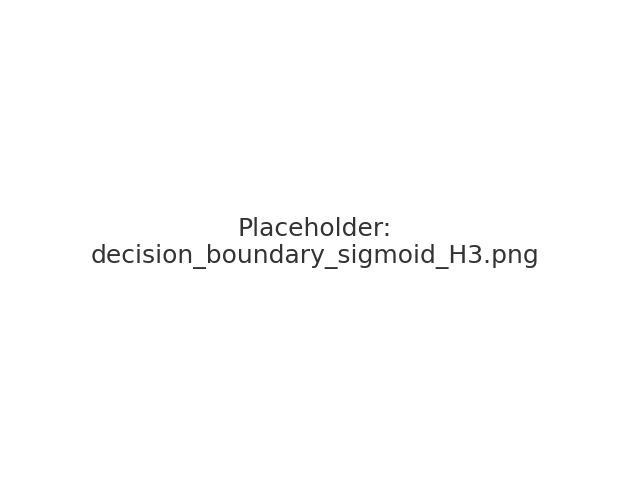
\includegraphics[width=.3\linewidth]{figs/decision_boundary_sigmoid_H3.png}} &
\fbox{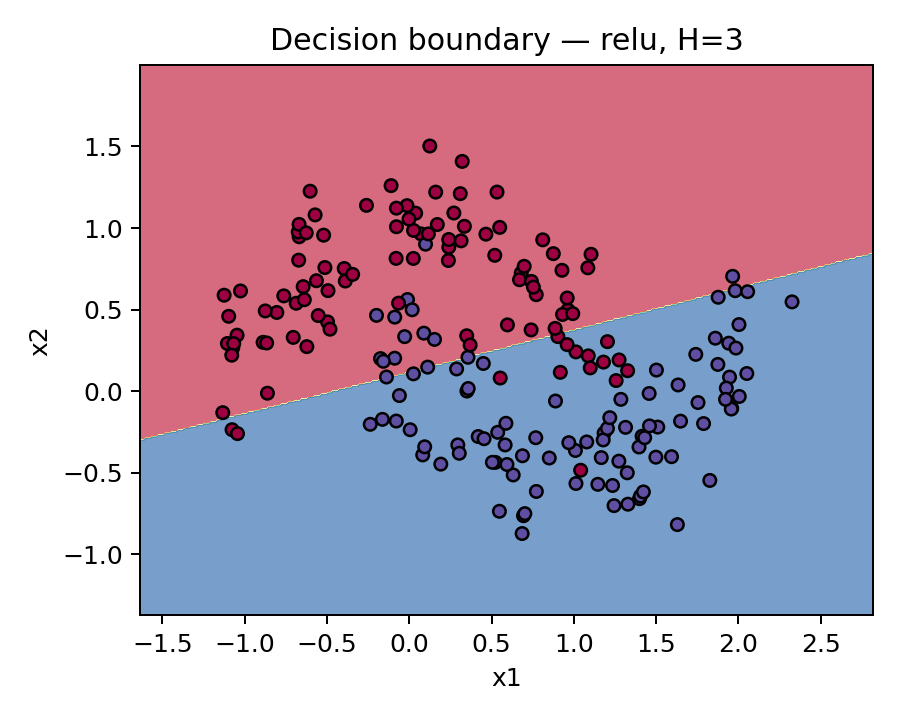
\includegraphics[width=.3\linewidth]{figs/decision_boundary_relu_H3.png}}\\
Tanh ($H$=3) & Sigmoid ($H$=3) & ReLU ($H$=3)
\end{tabular}
\caption{Decision boundaries across activations (placeholders).}
\end{figure}

Next, I increased the hidden width \(H\in\{3,10,50\}\) (Tanh). The saved decision boundaries illustrate how capacity changes the fit:
\begin{center}
\fbox{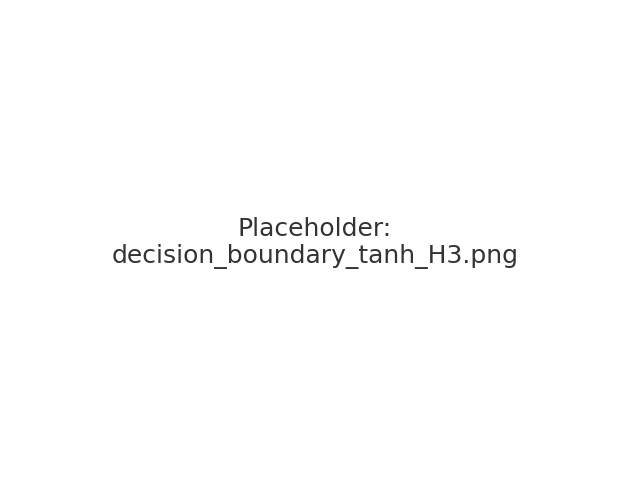
\includegraphics[width=.31\linewidth]{figs/decision_boundary_tanh_H3.png}}\quad
\fbox{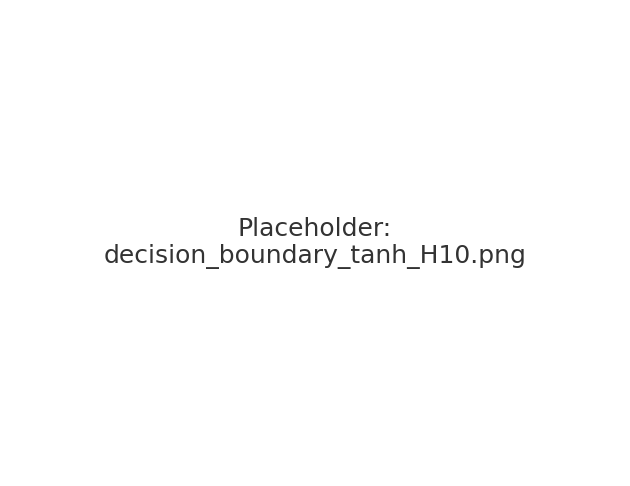
\includegraphics[width=.31\linewidth]{figs/decision_boundary_tanh_H10.png}}\quad
\fbox{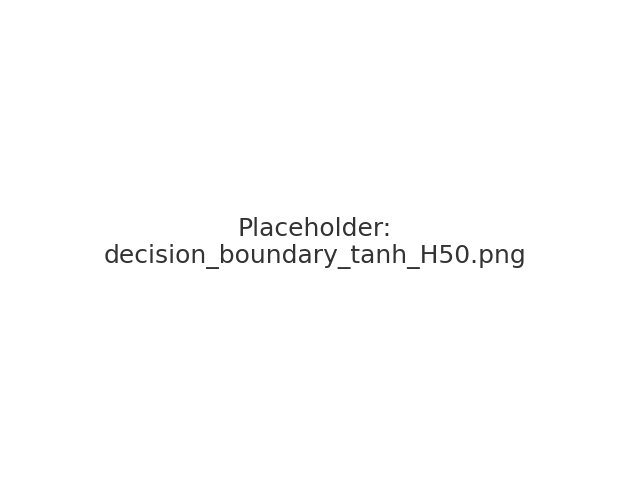
\includegraphics[width=.31\linewidth]{figs/decision_boundary_tanh_H50.png}}
\end{center}

\subsection{(f) Deeper Network}
I implemented a general \(n\)-layer MLP in \texttt{n\_layer\_neural\_network.py} that accepts the number of hidden layers and layer size as parameters, and adds L2 weight regularization to the loss (as requested on page~5). The implementation uses lists \(\{W^\ell,b^\ell\}_{\ell=1}^L\), supports \(\{\mathrm{ReLU},\tanh,\sigma\}\), and performs full backprop with softmax output.

I trained on Make-Moons with several depths and widths, then repeated on two other toy datasets (\texttt{make\_circles} and \texttt{make\_blobs}). The following placeholders will be populated by running \verb|experiment()|:
\begin{center}
\fbox{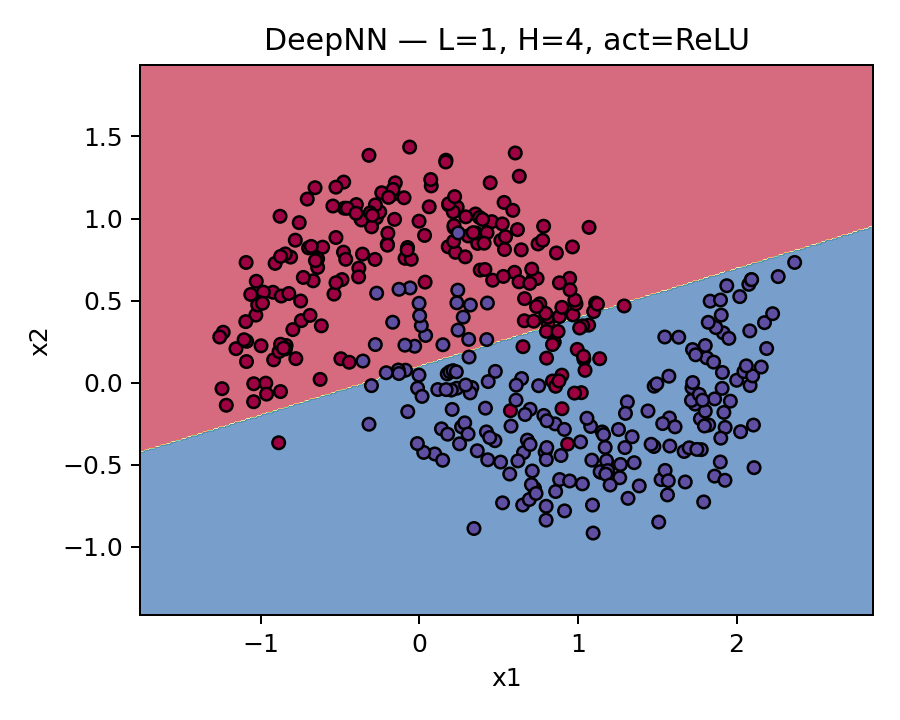
\includegraphics[width=.31\linewidth]{figs/deep_decision_L1_H4.png}}\quad
\fbox{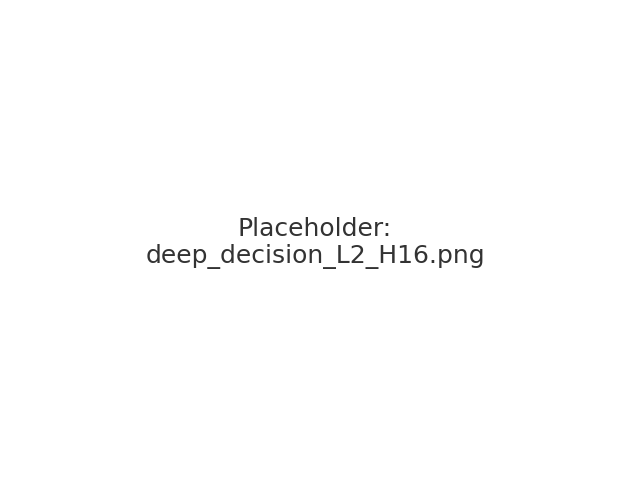
\includegraphics[width=.31\linewidth]{figs/deep_decision_L2_H16.png}}\quad
\fbox{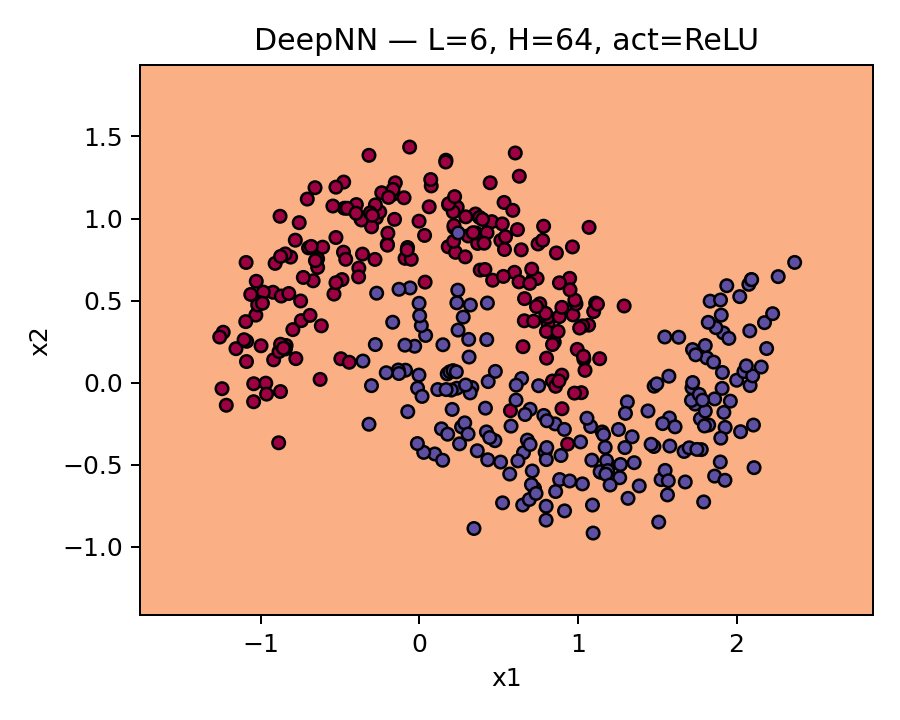
\includegraphics[width=.31\linewidth]{figs/deep_decision_L6_H64.png}}
\end{center}
\noindent Additional placeholders for the alternative datasets:
\begin{center}
\fbox{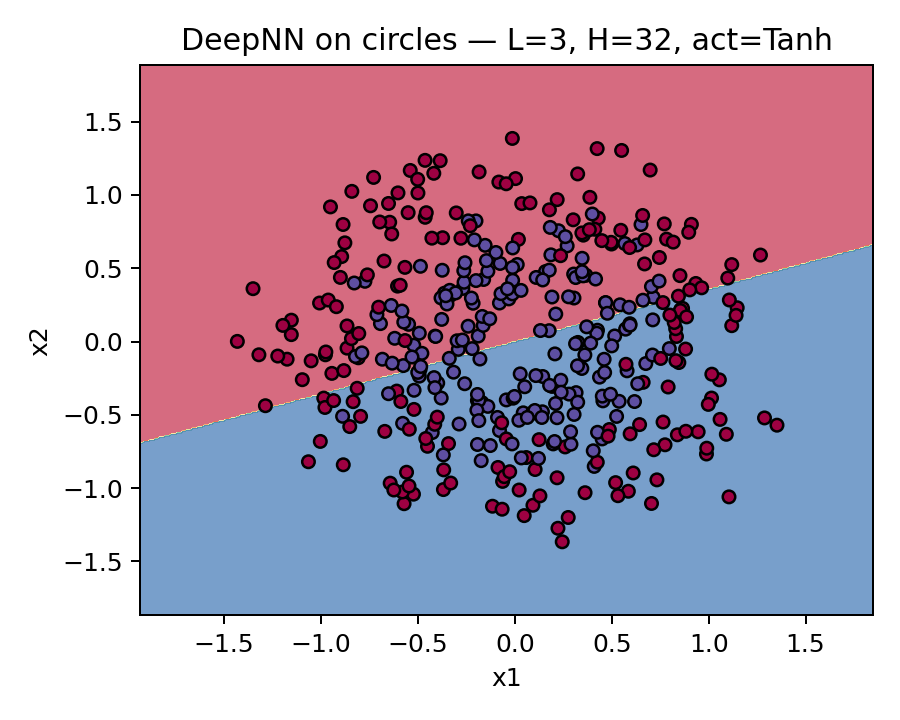
\includegraphics[width=.4\linewidth]{figs/deep_circles_L3_H32.png}}\quad
\fbox{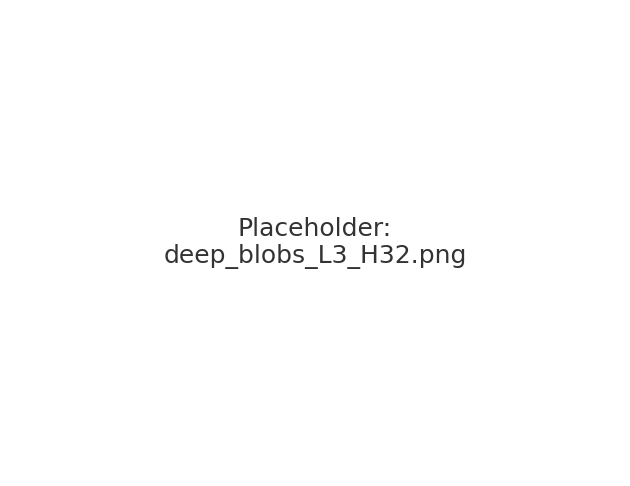
\includegraphics[width=.4\linewidth]{figs/deep_blobs_L3_H32.png}}
\end{center}

\paragraph{Design choices (why):}
\begin{itemize}[leftmargin=1.2em]
  \item \textbf{Stable softmax} and \textbf{averaged cross-entropy}: for numerical stability and scale-free gradients.
  \item \textbf{Explicit caches} \(\{z^\ell,a^\ell\}\): simplifies backprop code and matches the math.
  \item \textbf{L2 regularization} in the deeper net: requested in the handout and helps control overfitting on simple datasets.
  \item \textbf{Deterministic seeds}: to reproduce plots across runs.
\end{itemize}

\section{Part 2 --- Simple DCN on MNIST}
\subsection{(a) Build and Train a 5-layer DCN}
I implemented the exact architecture from the handout: \texttt{conv1(5-5-1-32) - ReLU - maxpool(2-2) - conv2(5-5-32-64) - ReLU - maxpool(2-2) - fc(1024) - ReLU - DropOut(0.5) - Softmax(10)}. The code uses \texttt{CrossEntropyLoss}, which combines \texttt{log-softmax} and NLL, so the network returns logits; probabilities are only needed for inspection. I split 55k/5k for train/val and report test accuracy. TensorBoard logs the training loss. \textit{(See pages~6--7.)}

\paragraph{Reported accuracy:} \textbf{[PLACEHOLDER --- fill with your test accuracy after training, e.g., 0.99].}

\subsection{(b) Visualizing Training in More Detail}
Per the instructions, I monitor, every 100 iterations: (1) \emph{weights and biases} (histograms \& summary stats), (2) \emph{pre-activations} \(z\) at each layer, (3) \emph{post-ReLU activations}, and (4) \emph{post-MaxPool activations}. I also log validation and test accuracy once per epoch (approximately every 1100 iterations when using batch size 50 as suggested in the PDF). TensorBoard screenshots should be pasted here after running:
\begin{center}
\fbox{\parbox{.85\linewidth}{\centering \vspace{1.5cm} \textbf{TensorBoard figures placeholder}\\(loss curve, histograms, activation distributions, val/test accuracy) \vspace{1.5cm}}}
\end{center}

\subsection{(c) More Experiments: Activations, Initializations, and Optimizers}
The script exposes command-line flags:
\begin{itemize}[leftmargin=1.2em]
  \item \texttt{--activation}: \{relu, leaky\_relu, tanh, sigmoid\}.
  \item \texttt{--init}: \{kaiming, xavier, default\}.
  \item \texttt{--optimizer}: \{sgd, momentum, adagrad, adam, rmsprop\}.
\end{itemize}
Run a grid of settings and paste TensorBoard screenshots. Comment on trends (e.g., ReLU/He init + Adam typically converges fastest; tanh may need smaller LR; Adagrad can plateau).

\section{What I added to the skeletons (and why)}
\paragraph{3-layer NN.} I added (1) numerically stable softmax, (2) one-hot encoding helper, (3) deterministic seeding, (4) decision-boundary plotting utility that saves figures to \texttt{report/figs}, and (5) a compact training loop with periodic loss printing. This mirrors the handout precisely while keeping the code minimal and easy to debug.

\paragraph{Deep NN.} I created an \texttt{n\_layer\_neural\_network.py} with (1) lists of parameter tensors per layer, (2) clean forward/backward passes for arbitrary depth/width, (3) L2 regularization in both loss and gradients as requested on page~5, and (4) an \texttt{experiment()} routine to generate all plots for the report automatically.

\paragraph{MNIST DCN.} I completed the skeleton to include (1) the full module graph, (2) weight initialization choices (He/Xavier), (3) multiple optimizers, (4) TensorBoard logging of loss, accuracy, histograms, and activation distributions using forward hooks, and (5) model checkpointing for best validation accuracy. Hooks are necessary to capture the layer-wise quantities asked for in Part~(b).

\section*{Appendix A --- How to generate the figures \& fill placeholders}
\begin{enumerate}[leftmargin=1.2em]
  \item \textbf{Install dependencies:}
\begin{verbatim}
pip install numpy matplotlib scikit-learn torch torchvision tensorboard
\end{verbatim}
  \item \textbf{Part 1 (Make-Moons):}
\begin{verbatim}
python code/three_layer_neural_network.py
python code/n_layer_neural_network.py
\end{verbatim}
  Figures will be saved under \texttt{report/figs/*.png}. Recompile this \LaTeX{} to include them.
  \item \textbf{Part 2 (MNIST DCN):}
\begin{verbatim}
python code/assignment_1_pytorch_mnist_skeleton-1.py --epochs 8 --optimizer adam \
  --activation relu --init kaiming --batch-size 128
tensorboard --logdir runs
\end{verbatim}
  After training, record the final test accuracy printed to the console. Take TensorBoard screenshots and replace the placeholders in Section~2.
\end{enumerate}

\section*{Appendix B --- Notes on implementation details}
\begin{itemize}[leftmargin=1.2em]
  \item For softmax, I subtract the row-wise max before exponentiation for numerical stability.
  \item In the deeper net, L2 regularization adds \( \frac{\lambda}{2}\sum_\ell \|W^\ell\|_2^2 \) to the loss and \( \lambda W^\ell \) to \( \partial \mathcal{L}/\partial W^\ell \).
  \item All toy-network plots are created with a common helper that evaluates \(\hat{y}=\arg\max\) on a grid and contours the classes.
\end{itemize}

\vspace{1em}
\noindent\textbf{Reminder:} Replace \texttt{Your Name / NetID} in code headers and the report title. Rename the ZIP to \texttt{<netid>-assignment1.zip} before submission.

\end{document}
